\documentclass{report}
\usepackage[14pt]{extsizes}
\usepackage[utf8]{inputenc}
\usepackage{graphicx}
\usepackage{textcomp}
\usepackage[french]{babel}
\usepackage{hyperref}
\usepackage{minted}
\usepackage{hyperref}


% Title Page
\title{Projet de fin d'études : le Robot Hermes}
\author{Rémi Dulong \and{Client : Claude Villard (Direction des formations)}
\and{Tuteur : Daniel Ranc}}

\date{Septembre 2017 - Janvier 2018}

\begin{document}

\begin{titlepage}
  \centering
  \vfill
  {\bfseries \Huge
      Rapport de projet de fin d'études : \\
  }
  {\huge
      \textit{Le Robot Hermes}\\
      Rémi Dulong\\
      Client : Claude Villard (Direction des formations)\\
      Tuteur : Daniel Ranc\\
      \vskip2cm
      Septembre 2017 - Janvier 2018\\
  }
  \vfill

  \vfill
  \vfill
\end{titlepage}

  \newpage

  \begin{abstract}
      {Ce rapport est le résultat d'un projet de fin d'études, dans le cadre de
       la voie d'approfondissement "Systèmes embarqués et objets communicants"
       de Télécom SudParis.}
  \end{abstract}

  \tableofcontents
  \newpage

\chapter{Objectif du projet}

  \section{Le projet Hermes}

    {Le projet Hermes est la continuité d'un projet initié en Janvier 2017 et
    qui a été porté par deux équipes de projet Cassiopée l'an dernier. L'Objectif
    est de créer de toutes pièces une plate forme robotisée multifonctions, dont
    une des fonctions serait par exemple l'accueil et le guidage de personnes dans
    l'enceinte de notre campus. Le projet Cassiopée s'est terminé en Juin 2017,
    avant que je ne reprenne la suite du projet en Septembre, ce projet étant pleinement
    compatible avec le domaine d'expertise de ma voie d'approfondissement en
    Systèmes Embarqués. Cette plate forme robotisée est une demande du département
    Direction des Formations de Télécom SudParis, et plus particulièrement de
    Monsieur Claude Villard, directeur des formations de l'école.}

    \section{Bilan des projets Cassiopée}

    {Mon projet de fin d'études étant la suite directe de notre travail lors des
     projets Cassiopée, je vais commencer par définir le point de départ de mon travail :}

     \subsubsection{La partie Hardware}

     {Un des deux projets Cassiopée s'était consacré à la réalisation physique
     du robot, c'est-à-dire la conception et la réalisation de la mécanique et
     de l'électronique. Nous avions établi un cahier des charges permettant de
    proposer une base roulante robotisée évolutive, comportant les éléments
    insidpensables pour assurer sa mobilité partout dans le campus.}

    \subsubsection{La partie Software}

    {Afin de donner au robot les fonctionnalités nécessaires en terme d'interactions
    entre ses différents composants ainsi qu'avec son environnement, l'autre partie
    de l'équipe (dont je faisais partie) était responsable de la partie logicielle.
    Nous avons séparé ce travail en 4 grandes parties :}
    \begin{itemize}
      \item Le programme embarqué sur le robot, responsable de ses
      fonctionnalités de base (en particulier le déplacement).
      \item Une application Android permettant le contrôle du déplacement en direct
      \item Une application Web permettant le pilotage du robot à distance via internet
      \item Notre distribution Linux minimaliste embarquée (conçue à l'aide de Yocto).
      \newline
    \end{itemize}

    \subsubsection{Résultats de Cassiopée}

    {À la fin du projet Cassiopée, nous avions pu faire rouler la base du robot
    dans son mode de pilotage le plus simple, c'est à dire en pilotage direct (
    mode télécommandé). Cependant, nous avons pu remarquer des disfonctionnements
    pendant ce test. Tout d'abord, un souci d'origine inconnue a fait que nous avions
    détruit une des deux cartes électroniques responsables de l'alimentation d'un
    des deux moteurs de propulsion. Cette carte (conçue par nos soins et réalisée
    par un industriel) avait, pour la cloture des projets Cassiopée, été remplacée
    en urgence par une autre carte que nous avions dû réaliser "à la main"
    (gravure sur plaques en époxy cuivrées). Cela s'est traduit par une asymétrie
    considérable rendant le robot difficile à contrôler, même via la télécommande
    en direct. De plus, une partie des fonctionnalités nécessaires au robot n'ont
    pas pû être développées par manque de temps, comme par exemple l'implémentation
    des capteurs de proximité dans le programme de pilotage. Enfin, le robot avait
    été pensé avant tout pour être piloté à distance via l'interface Web, ce qui
    avait engendré des complications conséquentes pour acheminer les ordres d'un
    utilisateur jusqu'au programme pilote, notamment à cause de la contrainte du
    réseau wifi à utiliser dans l'école, Eduroam.}


    \section{Architecture du Robot}

    {Le système que nous avons développé est conçu selon l'architecture suivante :}

    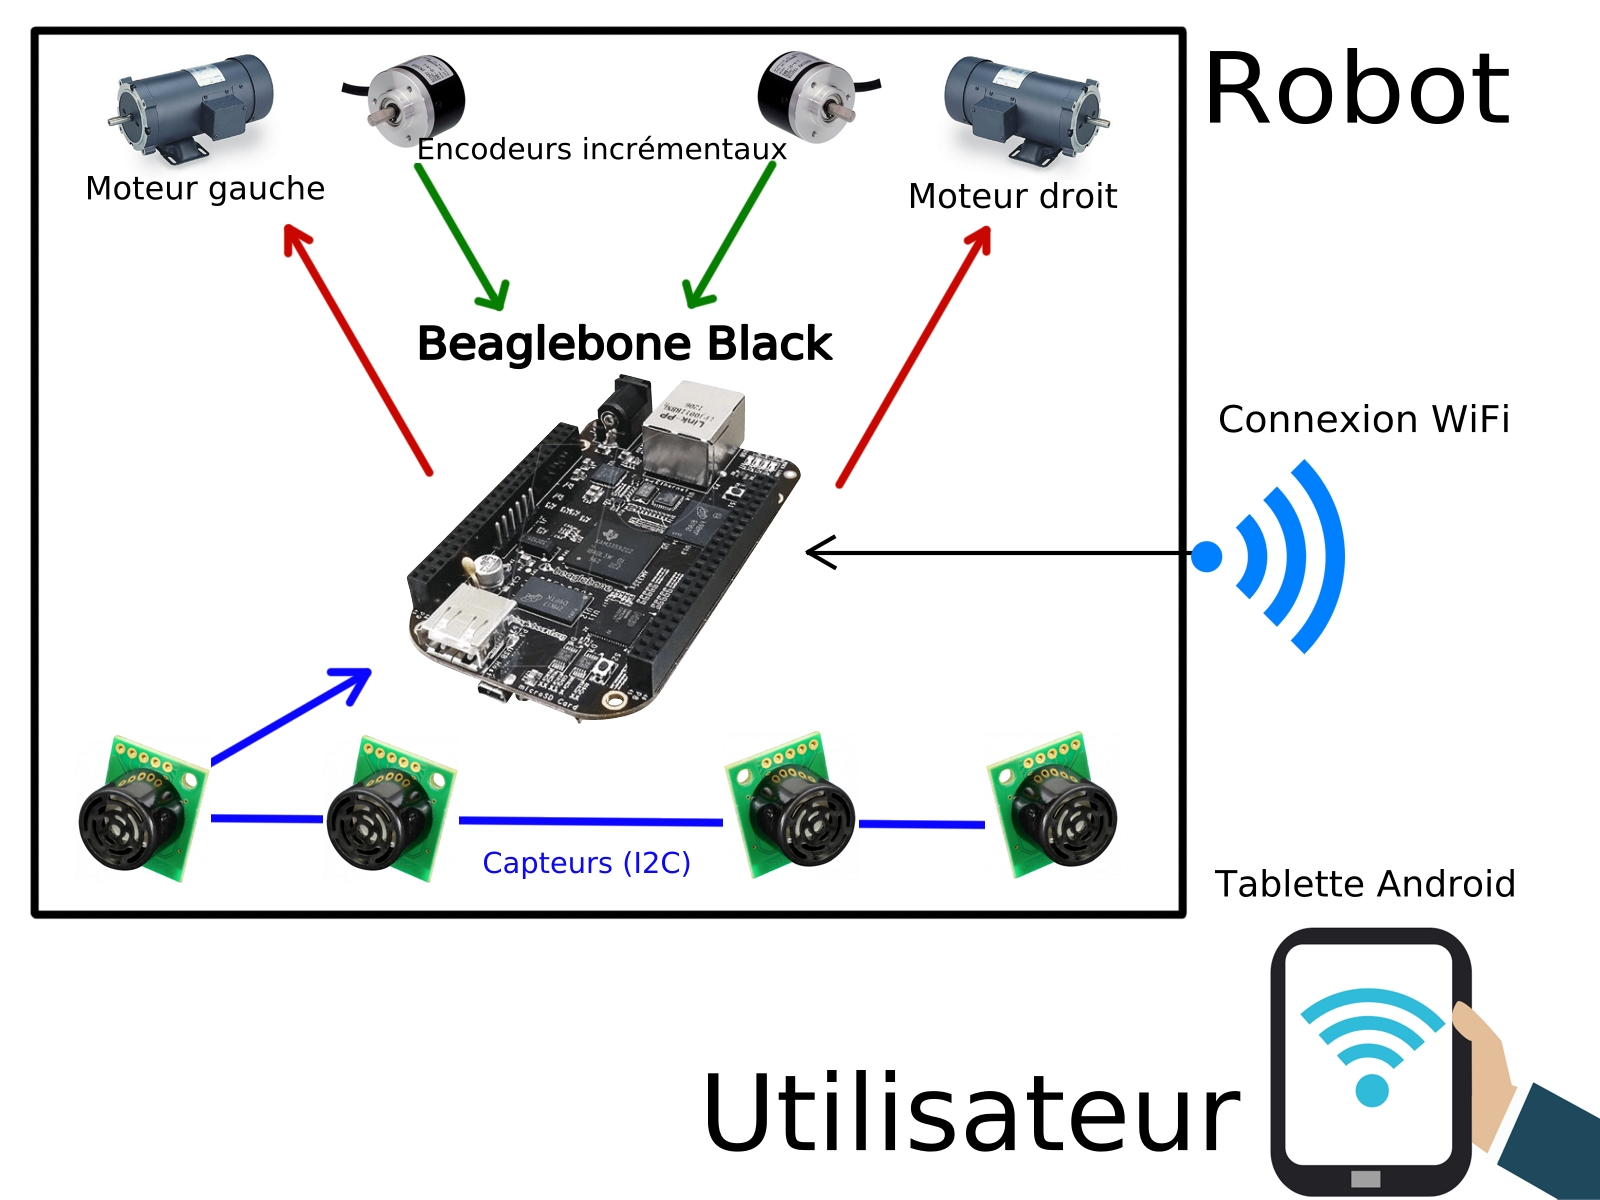
\includegraphics[scale=0.8]{img/hermes-archi.jpg}

    {Cette architecture est axée autour de deux éléments principaux :
    La Beaglebone Black, et la tablette Android.}

    \subsubsection{La Tablette Android}

    {La tablette Android est une des interfaces possibles pour l'interaction entre le robot
    et son utilisateur. En effet, il est également prévu de pouvoir contrôler le robot
    depuis une interface Web. Nous avions développé une application pour Android
    permettant le pilotage direct du robot (afin de tester le protocole de communication
    et la mobilité de la plateforme). Cependant, il s'agissait de la seule forme d'interaction
    possible en utilisant la tablette embarquée, ce qui était assez limité, et ne permettait
     pas encore le guidage d'un utilisateur dans le campus.}


    \section{Objectif du Projet de fin d'études}

    {L'objectif du PFE était de se focaliser davantage sur l'interaction directe
     entre les utilisateurs et le robot. Afin de pouvoir servir de guide, il
     fallait que le robot puisse recevoir des requêtes (de la forme "guide
     moi à l'amphi 10") de la manière la plus naturelle qui soit. Pour cela,
     nous avions choisi dans le cahier des charges d'utiliser une tablette
     tactile posée sur le robot. De plus, le projet devait rendre la base
     roulante utilisable en complétant les fonctionnalités qui n'avaient pas
     été implémentées lors du Cassiopée, en particulier la gestion des capteurs,
     et en tentant de corriger les anomalies constatées lors des tests à la fin
     du projet Cassiopée.}



  \chapter{Déroulement du PFE}

    \section{Intégration des capteurs}

        \subsection{Description des capteurs}

        \subsection{Mise en application}




    \section{Interaction avec les utilisateurs}

      {Afin de rendre les communication avec le robot les plus naturelles possible
      pour les utilisateurs, nous avons choisi d'utiliser de la reconnaissance vocale.
      Le fonctionnement du système de reconnaissance vocale est organisé selon
      un modèle client - serveur :}

      \subsection{Le client}
      {Le client que nous avons développé est une application Android. Ce choix n'est
      pas arbitraire, il permet en effet d'offrir des fonctionnalités particulièrement
      intéressantes :}

        \subsubsection{La simplicité de l'interaction}
        {L'utilisation d'une tablette, qu'elle soit accompagnée ou non de reconnaissance
        vocale, était déjà prévue au début du projet Hermes. En effet, elle permet
        d'obtenir une forme d'interaction simple pour l'utilisateur grâce à son écran tactile.
        Celui ci devait permettre notamment de montrer une carte du lieu, ainsi qu'un écran
        pour rechercher le bureau d'une personne sur le campus simplement à partir de son
        nom.}

        \subsubsection{L'API de Google}
        {Nous avons choisi d'utiliser une tablette sous Android, pour la simplicité de
        développement que cela implique, mais aussi pour avoir l'accès à l'API de reconnaissance
        vocale de Google. Cette API est composée de deux éléments complémentaires :}
        \begin{itemize}
          \item Le STT (Speech to text) : c'est l'outil capable de traduire le fichier
          audio contenant la requête vocale de l'utilisateur en une requête sous forme de
          chaîne de caractères.
          \item Le TTS (Text To Speech) : il s'agit de l'outil faisant le travail inverse.
          À partir d'une chaîne de caractères, le TTS génère un fichier audio contenant une
          voix synthétisée lisant la chaîne de caractères.
        \end{itemize}

        {L'avantage pour nous est que Google fournit cette API dans tous les appareils
        Android, et qu'elle peut être utilisée sans connexion Internet (ce qui est intéressant
        pour nous puisqu'il fallait que le mode d'interaction avec le robot ne soit pas
        tributaire de la présence d'une connexion wifi ou non).}

    \section{Le serveur}

    \subsection{Le choix de l'architecture matérielle}

    {Notre architecture avait pour objectif de tester les capacités d'un
    micro-ordinateur embarqué, afin de savoir si il était possible de gérer
    tous les éléments de base d'un robot depuis une unique carte. En effet,
    la plupart des architectures de robots que nous avions expérimenté pour l'instant
    (notamment au club de robotique de l'école) étaient constituées d'une carte
    dite "Bas niveau" et d'une carte dite "Haut Niveau". La première, souvent une carte
    de type Arduino, STM32, ou encore Teensy, avait pour rôle de gérer les
    problématiques de pilotage des moteurs et servomoteurs, tandis que la seconde
    permettait de gérer les problématiques de l'environnement du robot (grâce à l'interprétation
    des valeurs des capteurs) ainsi que la recherche de chemin (algorithme de Path Finding),
    mais aussi la communication avec l'utilisateur. Cette dernière, plus puissante,
    était souvent une Raspberry Pi. Cela nous obligeait donc à avoir
    un système de communication entre ces deux cartes, qu'il s'agisse d'une liaison série
    ou d'une connexion ethernet, transportant un protocole de communication simple réalisé
    par nos soins. Cependant, nous avions constaté des faiblesses qui pouvaient s'avérer
    critiques lorsque des déconnexions apparaissaient. Pour cette raison, nous voulions
    tester une autre forme d'architecture, en utilisant une seule et unique carte pour
    les applications haut et bas niveau.}

    \subsubsection{Fonctionnalités indispensables}

    {Afin de choisir l'ordinateur utilisé, nous avions deux contraintes principales :
    tout d'abord, la carte devait être suffisamment puissante pour permettre
    d'accueuillir des programmes "haut niveau" tels qu'un algorithme de recherche de chemin
    (relativement coûteux en terme de puissance de calcul) ou encore différents
    serveurs, comme par exemple notre serveur python en charge du traitement des
    phrases de la reconnaissance vocale. Tout cela fonctionnant en simultané avec
    le programme responsable de l'asservissement du robot, lui aussi potentiellement
    gourmand en ressources de calcul, de par la fréquence d'asservissement qui se doit
    d'être suffisamment élevée pour permettre de bons déplacements de la plate forme.
    Aussi, cette première contrainte nous obligeait à utiliser un système d'exploitation
    permettant d'installer et d'executer des programmes complexes et divers. C'est pour
    cela (et parce que nous le connaissions suffisamment) que nous avions choisi
    d'utiliser Linux.}
    {Puis, il fallait que la carte électronique possède les fonctionnalités
    hardwares indispensables pour pouvoir l'interfacer directement avec notre matériel,
    et en particulier avec les encodeurs incrémentaux permettant de mesurer la
    vitesse et la distance parcourue par le robot. En effet, ces systèmes ont pour
    sortie un signal dont nous devons pouvoir déduire le déplacement du robot en
    comptant simplement des fronts montants. Hors, ces fronts montants
    doivent êtres dénombrés grâce à des interruptions, il nous fallait donc choisir
    une carte embarquée disposant de gestion d'interruptions. Après quelques recherches,
    nous avions choisi d'utiliser une carte de type BeagleBone Black.}

    \subsubsection{La BeagleBone Black}

    {La carte Beaglebone black est un micro ordinateur destiné à être embarqué.
    Elle permet en théorie d'utiliser toutes les fonctionnalités requises par notre
    cahier des charges simultanément. Le processeur utilisé est un ARM Cortex A8
    cadencé à 1GHz, auquel on associe 512 Mo cd mémoire RAM DDR3, ce qui lui apporte
    des capacités de calcul supérieures à une Raspberry Pi. De plus, cette carte
    est plus adaptée à être utilisée dans des projets embarqués : elle possède
    beaucoup plus de GPIO, dont par exemple 3 bus I2C différents, contre un seul
    pour la Raspberry Pi 3. Dans la configuration actuelle du projet, un seul bus I2C
    peut suffir, cependant nous avions pensé à différentes améliorations qui pourraient
    demander des bus supplémentaires, ou davantage de GPIO.
    Enfin, la différence majeure avec une Raspberry Pi est que la Beaglebone
    possède des PRU (Programmable Real-Time Unit). Il s'agit en réalité de petits
    micro-controlleurs 32 bits indépendants situés dans la puce processeur de la carte,
    et qui permettent de faire cohabiter des fonctionnalités nécessitant du temps réel et un
    système d'exploitation qui ne l'est pas, dans notre cas, Linux. C'est cette différence
    fondamentale qui fait de la BeagleBone Black une carte bien plus adaptée à jouer
    le rôle d'ordinateur central unique pour un système robotisé.}

\begin{centering}
  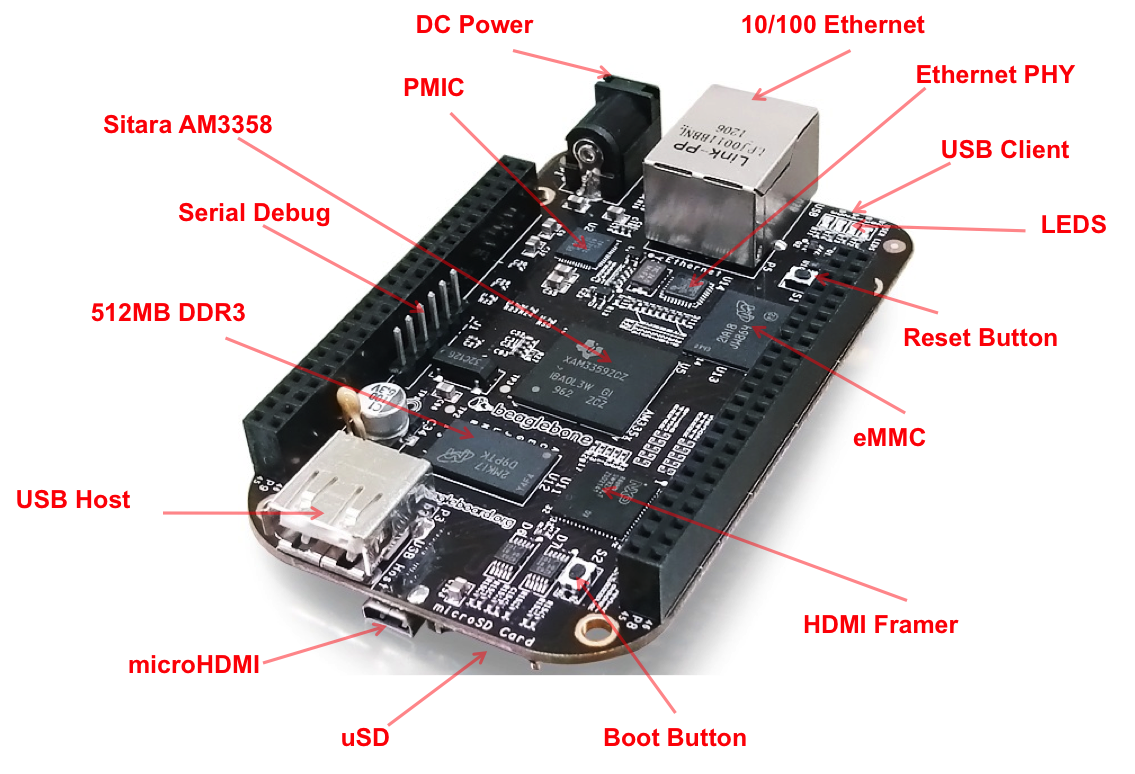
\includegraphics[scale=0.8]{img/black_hardware_details.png}
\end{centering}

    \section{L'architecture logicielle}

    \subsection{Le projet Yocto}
    {Comme nous souhaitions utiliser un système d'exploitation Linux, nous devions
    choisir quelle distribution de cet OS nous allions utiliser. Nous avions trois
    possibilités :}
    \begin{itemize}
      \item Utiliser un OS
    \end{itemize}




    {Les différentes fonctionnalités assurées par le serveur (c'est-à-dire la
    Beaglebone Black) sont réparties dans différents services. Dans le cadre de la
    nouvelle orientation du projet pour ce projet de fin d'études, à savoir l'utilisation
    du robot dans son mode "guidage" avec la tablette tactile comme interface avec
    l'utilisateur, il y a principalement deux programmes utilisés.}










\end{document}
